\head{Ноябрь}{Листок 10. Графы. Теория 2.}

\section{Эйлеровы и гамильтоновы обходы. Ориентированные графы.}

\begin{dfn}
    Граф называется \textit{эйлеровым}, если в нем существует цикл, проходящий по всем ребрам по одному разу, так называемый \textit{эйлеров цикл}. \textit{Полуэйлеров} (или \textit{почти эйлеров}) граф -- граф, в котором есть путь, проходящий по одному разу по каждому ребру.
\end{dfn}

\textit{\underline{Замечание}}: в частности любой эйлеров граф является почти эйлеровым, т.к. любой цикл является путём. Примером почти эйлеровых графов являются фигуры, которые можно нарисовать, не отрывая карандаша от бумаги и не проводя карандаш повторно по каким-либо линиям. 

\fbox{\begin{varwidth}{0.95\textwidth}
    \textbf{Теорема Эйлера (критерий эйлеровости графа)}. Граф эйлеров тогда и только тогда, когда он связен, и все его вершины имеют чётную степень. Граф полуэйлеров тогда и только тогда, когда он связен и имеет не более двух вершин с нечётной степенью.
\end{varwidth}}

\begin{dfn}
    Граф называется \textit{гамильтоновым}, если в нём существует замкнутый путь, проходящий через все вершины ровно по одному разу. Такой путь, соответственно, называют \textit{гамильтоновым} \textit{циклом}.
\end{dfn}

% \begin{figure}[H]
% \begin{minipage}{0.65\linewidth}\setlength{\parindent}{1.5em}
%     Многие головоломки сводятся к эйлеровости или гамильтоновости определенных графов. Эйлер придумал свою теорему в 1736 году в связи с задачей об обходе кенигсбергских мостов. Именно с теоремы Эйлера теория графов отсчитывает свою историю. Гамильтоновы путь, цикл и граф названы в честь ирландского математика сэра Уильяма Гамильтона, который в 1859 году впервые определил эти классы, исследовав задачу «кругосветного путешествия» по додекаэдру, узловые вершины которого символизировали крупнейшие города Земли, а рёбра – соединяющие их дороги. Играющий должен обойти все города и вернуться в исходный. 
% \end{minipage}
% \hfill
% \begin{minipage}{0.3\linewidth}
%     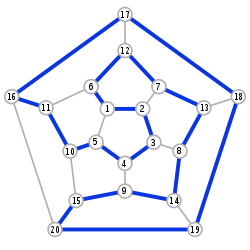
\includegraphics[width=0.95\columnwidth]{img/10.2 1 pyat.png}
% \end{minipage}
% \end{figure} 

\begin{wrapfigure}{R}{0.35\textwidth}
\centering
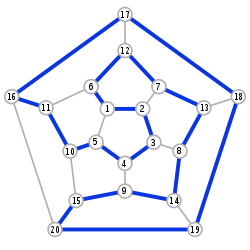
\includegraphics[width=0.3\textwidth]{img/10.2 1 pyat.png}
\end{wrapfigure}

Многие головоломки сводятся к эйлеровости или гамильтоновости определенных графов. Эйлер придумал свою теорему в 1736 году в связи с задачей об обходе кенигсбергских мостов. Именно с теоремы Эйлера теория графов отсчитывает свою историю. Гамильтоновы путь, цикл и граф названы в честь ирландского математика сэра Уильяма Гамильтона, который в 1859 году впервые определил эти классы, исследовав задачу «кругосветного путешествия» по додекаэдру, узловые вершины которого символизировали крупнейшие города Земли, а рёбра – соединяющие их дороги. Играющий должен обойти все города и вернуться в исходный. Справедливости ради следует отметить, что уже до этого была задача, сводящаяся к гамильтоновости некоторого графа, а именно задача обхода конем всех полей шахматной доски с возвращением в исходную клетку. Эта задача была в своё время успешно решена Эйлером. На рисунке изображен граф додекаэдра Гамильтона.

\begin{figure}[H]\begin{minipage}{0.3\linewidth}
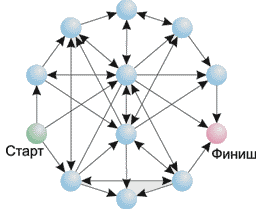
\includegraphics[width=0.95\columnwidth]{img/10.2curse.png}
\end{minipage}
\hfill
\begin{minipage}{0.69\linewidth}\setlength{\parindent}{1.5em}
    \begin{dfn}
    Пусть $n$ -- количество вершин в данном графе. Если степень каждой вершины не менее, чем $\dfrac{n}{2}$, то граф называется \textit{графом Дирака}.
    \end{dfn}
    \begin{ques}
        Почему граф Дирака связен?
    \end{ques} 
    (На рисунке изображён граф из задачи поиска гамильтонова пути с помощью ДНК--вычислений.)
    \\
    Для гамильтоновости графов в отличие от эйлеровости не найдено простых критериев. Тем не менее существует много достаточных условий. Приведём некоторые из них.
\end{minipage}
\end{figure}

\fbox{\begin{varwidth}{0.95\textwidth}
    \textbf{Теорема Поша.} Пусть граф имеет p вершин, где $p \geq 3$. Если для всякого $n$ такого, что $1 \leq n \leq \dfrac{p - 1}{2}$, число вершин со степенями, не превосходящими $n$, меньше чем $n$, и для нечётного $p$ количество вершин степени $\dfrac{p - 1}{2}$ не превосходит $\dfrac{p - 1}{2}$, то такой граф гамильтонов.
    \\
    \textbf{Теорема Оре.} Если граф имеет $p$ вершин, где $p > 2$ и сумма степеней несмежных вершин не меньше $p$, то граф гамильтонов. 
    \\ 
    \textbf{Теорема Дирака.} Если граф имеет $p$ вершин, где $p > 2$ и степень любой вершины не меньше $\dfrac{p}{2}$, то граф гамильтонов.
\end{varwidth}}

\newpage

\begin{ques}
    Является ли дерево эйлеровым графом?
\end{ques}

\begin{ques}
    Является ли дерево гамильтоновым графом?
\end{ques}

\begin{dfn}
    Граф называется \textit{двусвязным}, если между любыми двумя вершинами существует два непересекающихся по вершинам (кроме начала и конца) пути.
\end{dfn}

\textit{\textbf{Утверждение.}} Гамильтонов граф двусвязен.

\begin{dfn}
    \textit{Тэта-графом} называется граф из двух вершин степени 3 и трёх непересекающихся простых путей, соединяющих их, причём длина каждого из путей не меньше 2.
\end{dfn}

\fbox{\begin{varwidth}{0.95\textwidth}
    \begin{thrm}
        Каждый негамильтонов двусвязный граф содержит тэта--подграф.
    \end{thrm}
\end{varwidth}}

Задачи, в которых нужно доказать отсутствие гамильтонова цикла, часто сводятся к поиску инварианта или какой-нибудь величины на вершинах, которая известным образом изменяется при переходе от вершины к смежной вершине. Как, например, шахматная раскраска в следующем примере.

\begin{thm}
    Докажите, что шахматный конь не может обойти доску 5 на 5 и вернуться в исходную клетку.
\end{thm}

\begin{prf}
    Каждым ходом конь встаёт на клетку другого цвета. Так как всего ходов 25 -- нечётное число, то последним ходом он должен встать на клетку, не совпадающую по цвету с начальной. Противоречие.
\end{prf}

\begin{dfn}
    Граф, в котором рёбра снабжены стрелками, называется ориентированным. Полный граф, в котором каждое ребро снабжено ориентацией (стрелкой), называется \textit{полным ориентированным графом }или \textit{турниром}.
\end{dfn}

\begin{dfn}
    \textit{Исходящей степенью} вершины в ориентированном графе называется количество рёбер, выходящих из данной вершины. \textit{Входящей степенью} вершины в ориентированном графе называется количество рёбер, входящих в данную вершину.
\end{dfn}
\hfill \break
Заметим следующий общий факт. Так как каждое ориентированное ребро имеет одно начало и один конец, то сумма всех исходящих степеней вершин равна количеству рёбер. Аналогично каждое ребро имеет один конец, поэтому сумма входящих степеней вершин равна количеству рёбер. Потому сумма исходящих степеней вершин равна сумме входящих степеней вершин.

\begin{thm}
    В однокруговом турнире по настольному теннису каждый участник одержал четыре победы. Сколько человек участвовало в турнире? (Ничьих в теннисе не бывает).
\end{thm}

\begin{prf}
    Обозначим участников за вершины графа. Если участник A выиграл у участника B, поставим стрелку от A к B. Переформулировка на язык графов: «В полном ориентированном графе из каждой вершины выходит четыре ребра. Сколько в нём вершин?».
    \\
    Пусть всего в графе $x$ вершин, у каждой из которых исходящая степень 4. Сумма исходящих степеней вершин -- $4x$, сумма входящих -- такая же. Так как общая степень каждой вершины одна и та же и равна $x – 1$, а исходящая равна 4, то входящая степень у всех вершин тоже одинакова. Значит, она тоже равна 4. Отсюда $x
    – 1 = 8$, и в турнире принимало участие 9 человек.
\end{prf}